\chapter{مقدمه}

\section{مقدمه}
در صنعت، نگهداری و تعمیرات\LTRfootnote{Maintenance} به تمام فعالیت‌هایی اطلاق می‌شود که بر روی ابزارهای صنعتی انجام می‌شود تا بهره‌وری و عمر این ابزارها افزایش یابد. در سال‌های اخیر، رویکردهای مختلفی برای انجام نگهداری مورد استفاده قرار گرفته است. روش‌های نگهداری زیر، از میان همه‌ی این رویکردها، بیشترین فراوانی استفاده در صنعت را دارند\cite{zhao2022review}:

\begin{itemize}

\item \textbf{نگهداری و تعمیرات اصلاحی\LTRfootnote{Corrective Maintenance}}: به جایگزینی قطعه خراب شده در سیستم می‌پردازد. در این رویکرد، تا زمانیکه فرایند جایگزینی قطعه معیوب به اتمام نرسد، سیستم غیرقابل بهره‌برداری است و تعمیر قطعات بعد از خرابی هزینه‌های قابل توجهی برای صاحبان صنعت به همراه دارد\cite{ran2019survey}.

\item \textbf{نگهداری و تعمیرات جلو‌گیرانه\LTRfootnote{Preventive Maintenance}}: سعی در پیش‌گیری از اتلاف زمان ناشی از توقف اضطراری دارد، اما در عوض ممکن است تعدادی از قطعاتی که هنوز عمر مفید دارند، دور ریخته شوند و اصراف در هزینه و قطعات مصرفی صورت گیرد\cite{ran2019survey}.

\item \textbf{نگهداری و تعمیرات پیش‌بینانه\LTRfootnote{Predictive Maintenance}}: سعی می‌کند مشکلات دو نوع نگهداری و تعمیرات مذکور را حل کند. با استفاده از این روش، زمان عملیاتی هر قسمت دستگاه تخمین زده می‌شود و قطعاتی که توسط سیستم مشکوک به خرابی در آینده هستند تعویض می‌گردند و بنابراین ابزارهای موجود در سیستم به صورت بهینه مورد استفاده قرار می‌گیرند و هزینه‌های تعمیرات بشدت کاهش می‌یابد\cite{zonta2020predictive, ran2019survey}.

\end{itemize}

بدلیل اینکه در نگهداری پیش‌بینانه قطعات در حال خرابی، پیش از وقوع خرابی شناسایی می‌شوند و ناکارآمدی آن بخش به کل سیستم آسیب نمی‌رساند، همانطور که در \cref{fig:maintenance_comparison} مشخص است، با استفاده از این نوع نگهداری، می‌توان مجموع هزینه‌های نگهداری و تعمیرات را به حداقل میزان ممکن رساند\cite{zonta2020predictive}.

\begin{figure}[!h]
\centerline{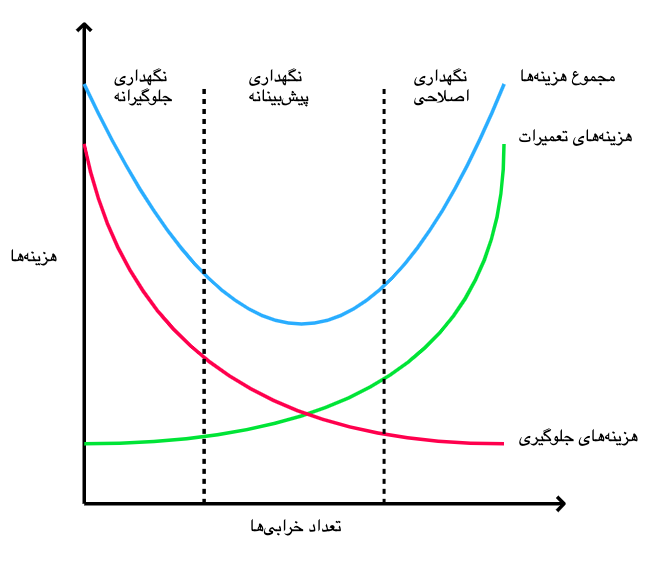
\includegraphics[width=.8\textwidth]{maintenance_comparison.png}}
\caption{مقایسه‌ی هزینه‌های انواع نگهد‌اری‌ها}
\label{fig:maintenance_comparison}
\end{figure}


\section{تعریف مسئله}
هدف از انجام این پروژه، پیاده‌سازی سیستمی برای اجرا کردن نگهداری پیش‌بینانه بر روی گره‌های موجود در یک اینترنت اشیاء\LTRfootnote{Internet of Things} به هم پیوسته است. رویکردهای مختلفی برای این منظور تا کنون توسط محققان ابداع و مورد استفاده قرار گرفته شده است. از جمله‌ی این موارد می‌توان به تحلیل لرزش\LTRfootnote{Vibration Analysis} اشاره کرد. برای پیاده‌سازی این سیستم همانطور که در \cref{fig:workflow} به تصویر آمده ‌است، نیازمند آنیم که داده‌های لرزش مربوط به گره‌ها را که توسط یک سیستم قابل اتکا\LTRfootnote{Reliable} جمع‌آوری شده است، دریافت کرده و با جدا کردن داده‌های پرت\LTRfootnote{Outlier Data}، از بین بردن تاثیر اختلال\LTRfootnote{Noise} ایجاد شده توسط گرانش و خرابی یا درست‌ کار نکردن حسگر\LTRfootnote{Sensor} اندازه‌گیری لرزش، استخراج ویژگی‌\LTRfootnote{Feature Extraction}های مناسب برای انجام تحلیل روی داده و درنهایت پیشنهاد دادن مدلی برای نحوه‌ی یادگیری ماشین\LTRfootnote{Machine Learning} و تحلیل و مقایسه‌ی داده‌های بدست‌آمده با داده‌های برچسب‌دار\LTRfootnote{Labeled Data}، عمر باقی‌مانده\LTRfootnote{Remaining Useful Lifetime}‌ی دستگاه‌های مختلف را پیش‌بینی کنیم و بر اساس اعداد بدست‌آمده، اقدامات مناسب را برای انجام مراقبت‌های دوره‌ای انجام دهیم و از تحمیل‌شدن هزینه‌های جانبی در آینده جلوگیری کنیم.

\begin{figure}[!h]
\centerline{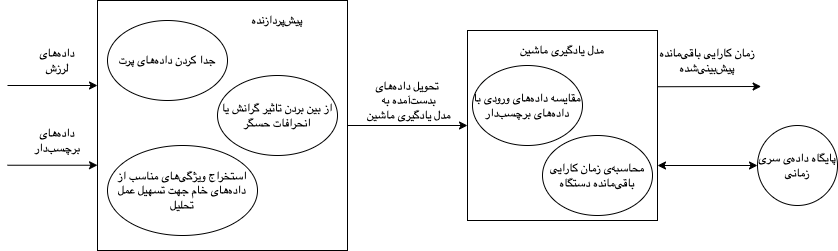
\includegraphics[width=1\textwidth]{workflow.png}}
\caption{نمودار جریان کار}
\label{fig:workflow}
\end{figure}


\section{کارهای مشابه}
